\section{dSPACE Unit}

A dSPACE unit is a multipurpose unit for implementing and testing controllers. The provided dSPACE unit contains a DS1103 PCC controller board.  % https://www.dspace.com/en/inc/home/products/hw/singbord/ppcconbo.cfm
The dSPACE unit is a platform that makes it possible to implement a control directly from simulink to the test plant. This is smart because almost every control engineering controller is designed without simulation, and therefor the controller is already implemented in simulink. This is also the case is this project. 

The provided dSPACE controller board is made for general motor control. The unit is fitted with both digital I/O, A/D converters, D/A converters and a CAN interface which is often used in motor applications, and also for the provided genset. 


\subsection{Implementation}
\label{dspace_unitv2}
% Opbygning start med at vise, hvad det er vi bruger hardware. Vis billeder også gå ind i software og beskriv bloggene 

This subsection will elaborate how to implement the controller on the dSPACE unit. Furthermore the software tool ControlDesk will be explained. 

As elaborated previously the controller will be implemented in simulink. To control the references for the AVR and governor through simulink a system block, which have been designed by dSPACE Real-Time Interface (RTI) \cite{dSPACE_software}, have been used. This block allows the user to send references to the AVR and governor through CAN bus. These system blocks are illustrated in \figref{fig:can_setup}:

\begin{figure}[H]
\centering
\includegraphics[width=1\textwidth]{rapport/billeder/cansetup}
\caption{System blocks for setting up CAN connection to the genset for voltage and frequency.}
\label{fig:can_setup}
\end{figure}    

The top module is used to set the frequency reference and the bottom is used to set voltage reference. The block called speed is used to set the wanted frequency in Hz for the output of the genset. To set the reference for voltage the block actVOLTAGE needs to be set at the desired output. The rest of the blocks are determent by the genset and the values can be found in the datasheet for the genset that will be tested on. 

To calculate the output in frequency and voltage, calculations done in simulink by Jesper Viese Knudsen, have been used. In \figref{fig:RMS_for_onePhase_simulink} it is illustrated how to calculated RMS voltage for one phase. 

\begin{figure}[H]
\centering
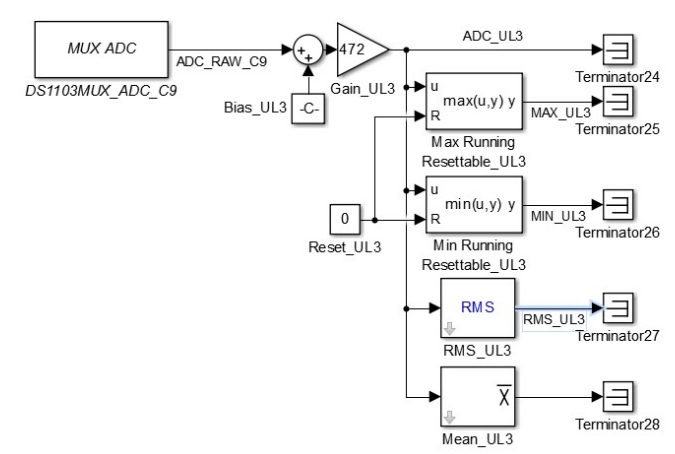
\includegraphics[width=0.8\textwidth]{rapport/billeder/RMS_for_onePhase_simulink}
\caption{System blocks for calculating RMS voltage for one phase.}
\label{fig:RMS_for_onePhase_simulink}
\end{figure} 

The output of block RMS\_UL3 will be used to calculate one phase of the voltage. The output will be in rms voltage, and to calculate all three phases, three setups like the on in \figref{fig:RMS_for_onePhase_simulink} will be used. 

In \figref{fig:CAN_frequency} an illustration of the system blocks to calculate frequency is shown. 

\begin{figure}[H]
\centering
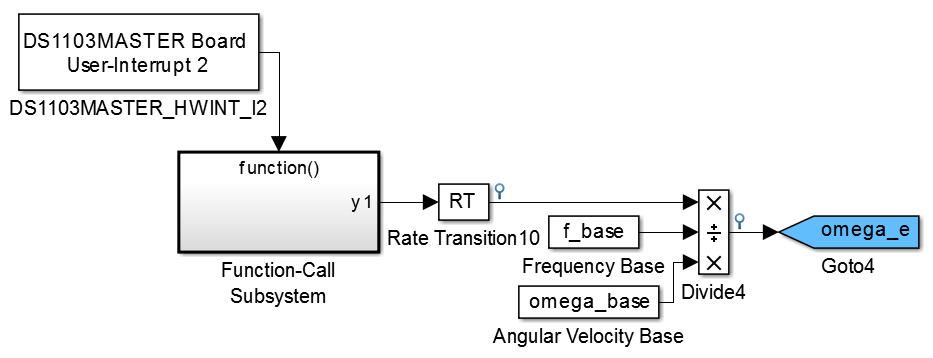
\includegraphics[width=0.8\textwidth]{rapport/billeder/CAN_frequency}
\caption{System blocks for calculating frequency.}
\label{fig:CAN_frequency}
\end{figure} 

The output of Divide4 is the frequency in rad/s which will be used to see if the frequency of the genset is stable with the controller designed in \secref{system_design_implementation}. 
It calculates the frequency through an sfunction in matlab, which uses interrupts from the tachometer placed inside the engine, to generate an input to this sfunction. By that a output in frequency will be calculated. 


These blocks have been added together with the controller designed in \secref{system_design_implementation} and the full implementation is illustrated in \figref{fig:full_implementation}.
\begin{figure}[H]
\centering
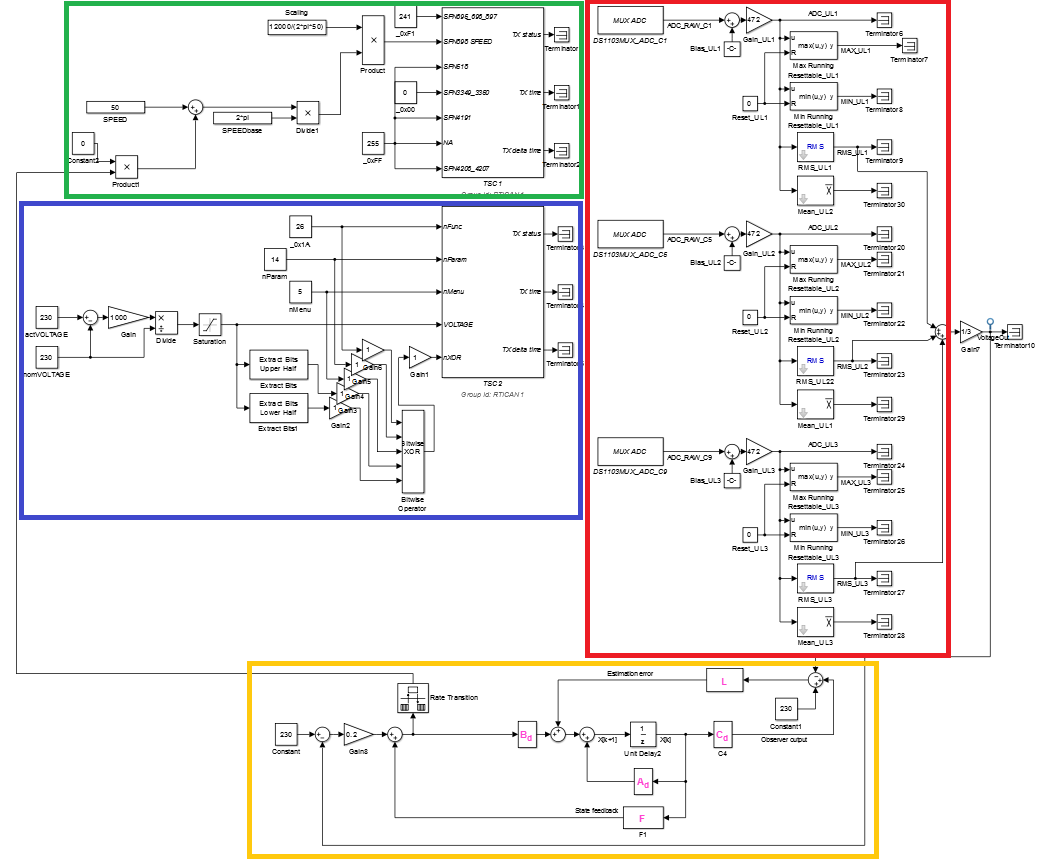
\includegraphics[width=1.1\textwidth]{rapport/billeder/full_implementation}
\caption{Full implementation on the dSPACE unit. In the green box the transformation from frequency reference to CAN bus commando for the governor is made. In the blue box the transformation from voltage reference to CAN bus commando for the AVR is made. The red box is transformation to RMS voltage. The yellow box is the controller.}
\label{fig:full_implementation}
\end{figure} 

To compile the simulink file the following code needs to be runned in matlab:

\begin{lstlisting}
rti_build('CA7_full_system')
\end{lstlisting}

When it has compiled it will be uploaded to the dSPACE unit. 

To analyses the output of the blocks in \figref{fig:full_implementation} ControlDesk have been used. ControlDesk is a software used to measure realtime data and gives the possibility to change values realtime. In this project it has been used to adjust the gain to find the parameter that fits the genset the most as in \secref{app:controller_test} Furthermore it has been used to track the output frequency and voltage, the states of the observer and the output of the observer. This gives the possibility to investigate if the values, an example is to look at the states of the observer to see if they are going towards infinity or towards zero which makes the search for error faster. 

 
% Furthermore the hardware that will used in this project will be shown and described.  

% The dSPACE unit is connected to a PC that runs simulink, matlab and ControlDesk these software tools will be elaborate later in this subsection. Furthermore, it is connected to several boards that are mounted on a wooden plate. These boards enable the dSPACE unit to measure voltage and current, communicate over CANbus and use calculated the electric frequency of the genset.  

% \begin{figure}[H]
% \centering
% \begin{subfigure}{.5\textwidth}
%   \centering
%   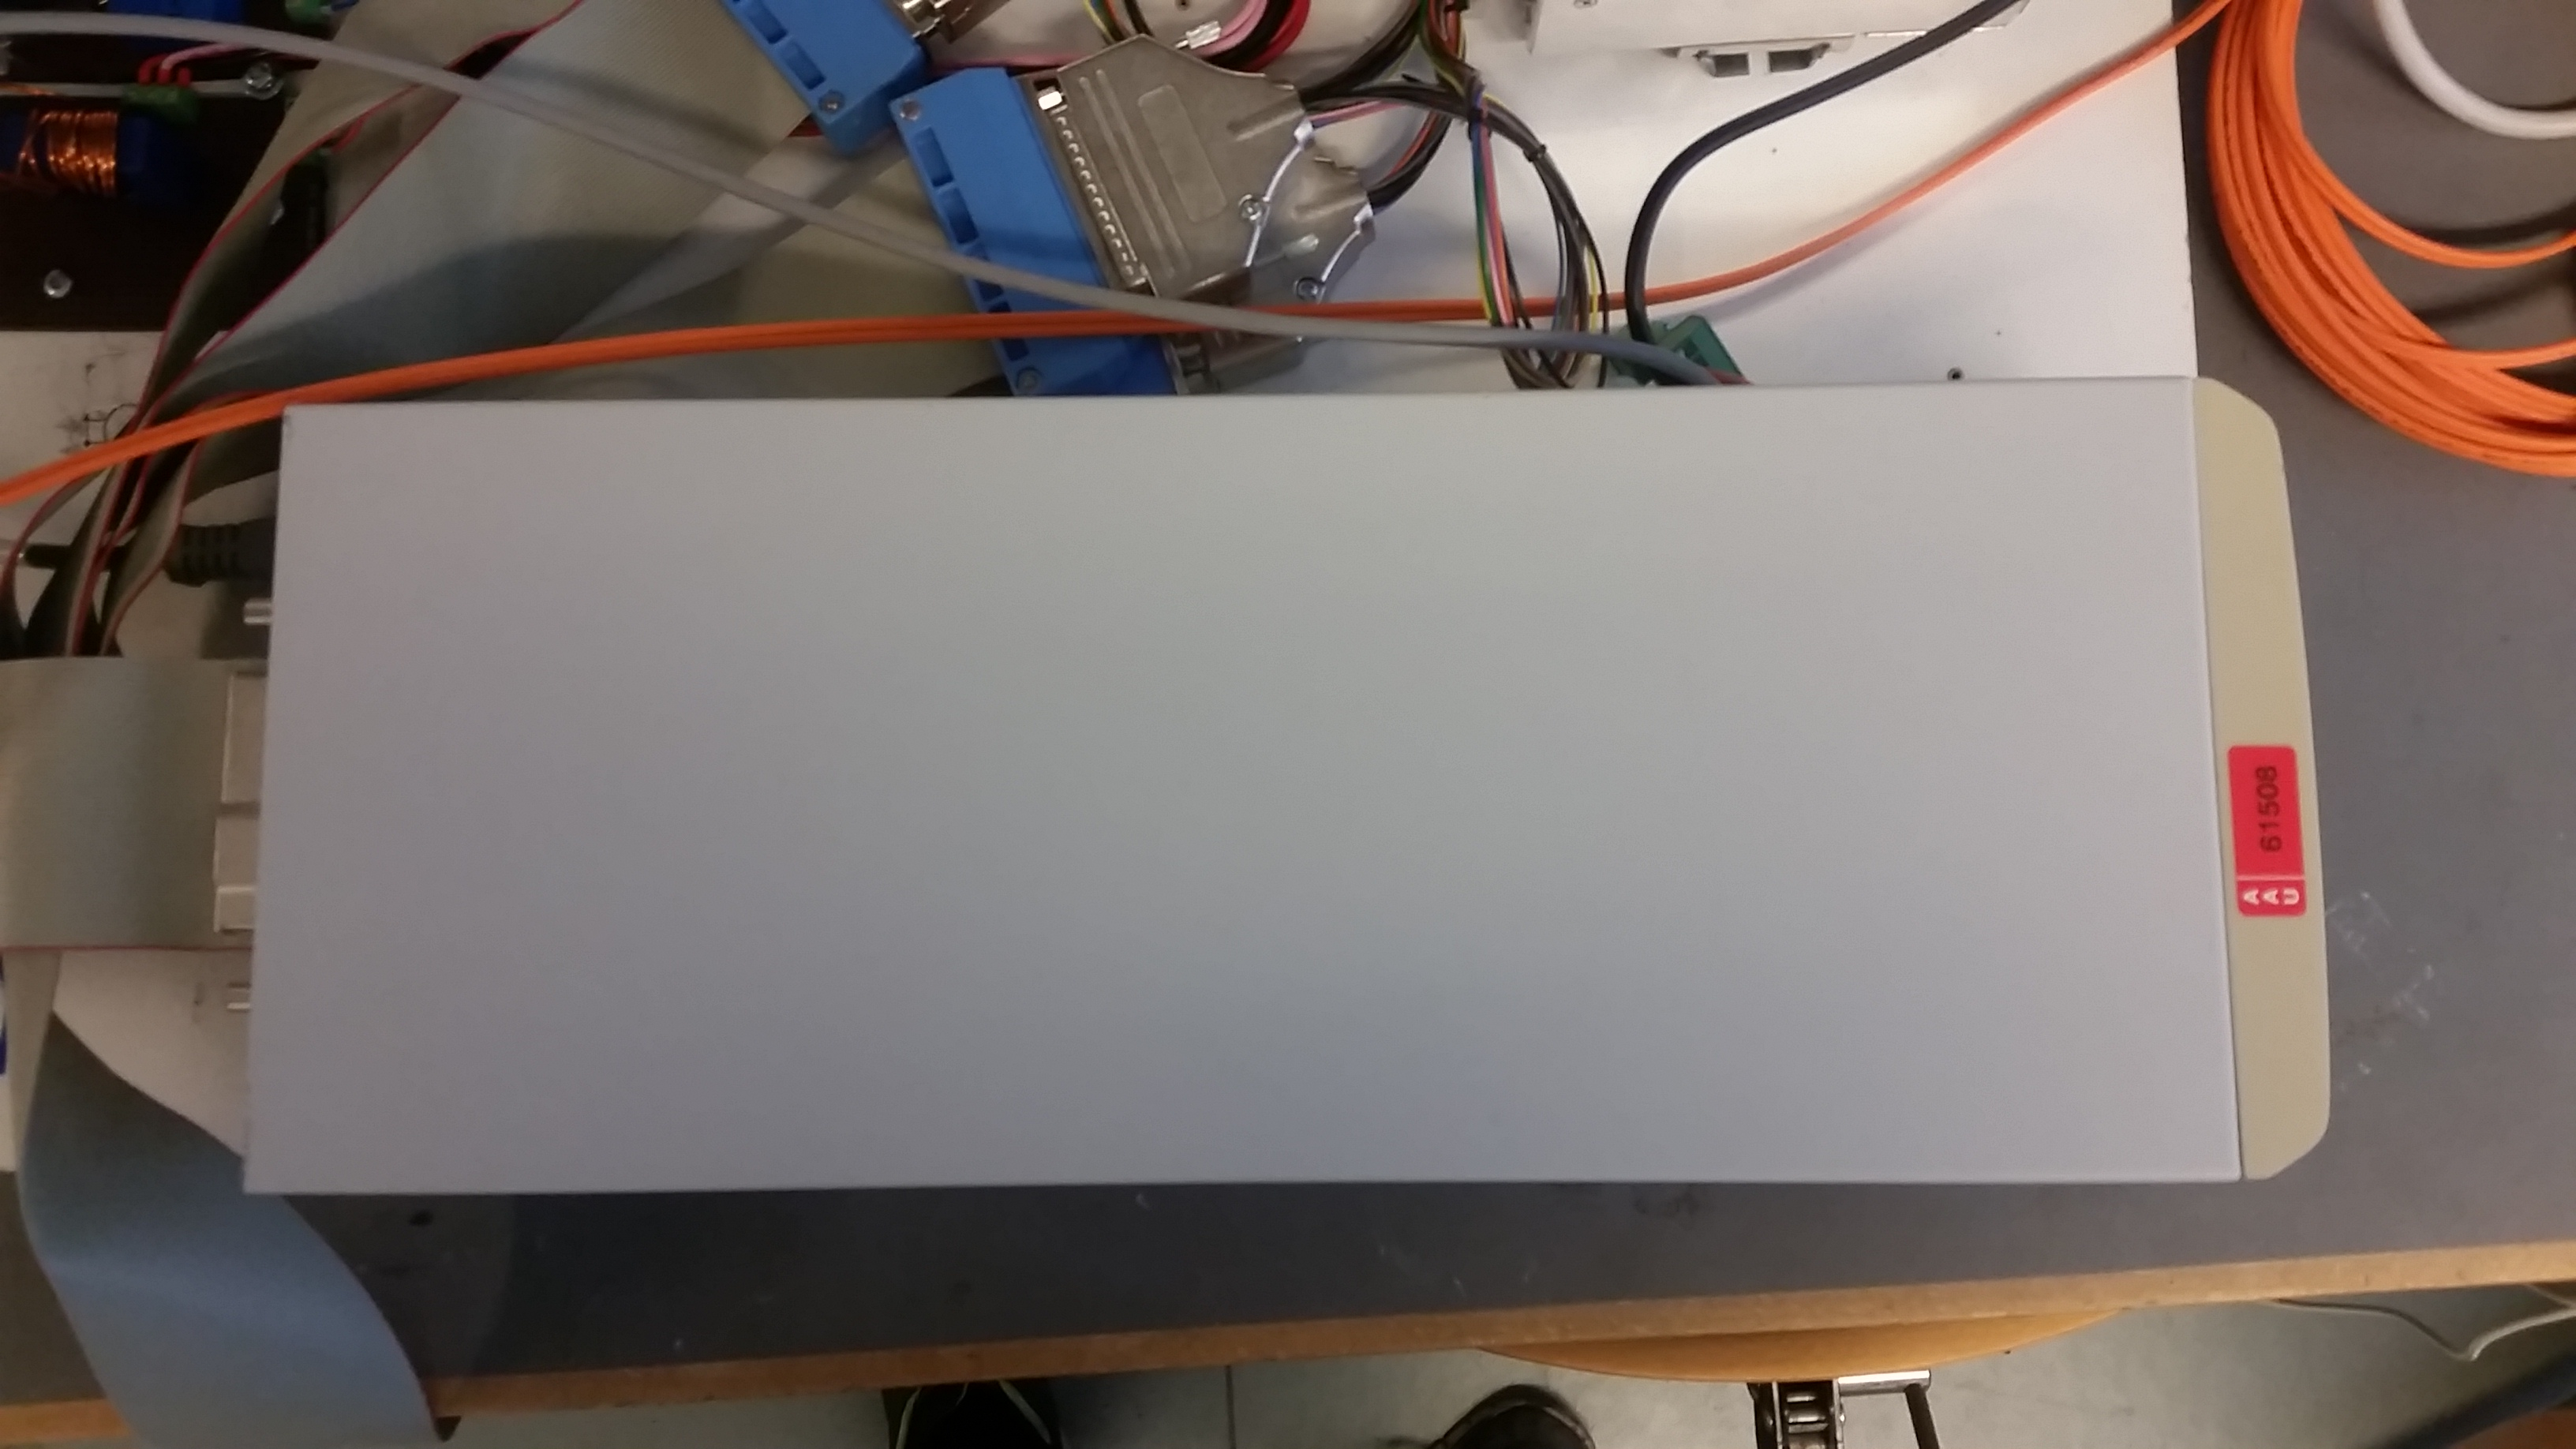
\includegraphics[width=0.75\textwidth]{rapport/billeder/dspace_unit}
%   \caption{}
% \end{subfigure}%
% \begin{subfigure}{.25\textwidth}
%   \centering
%   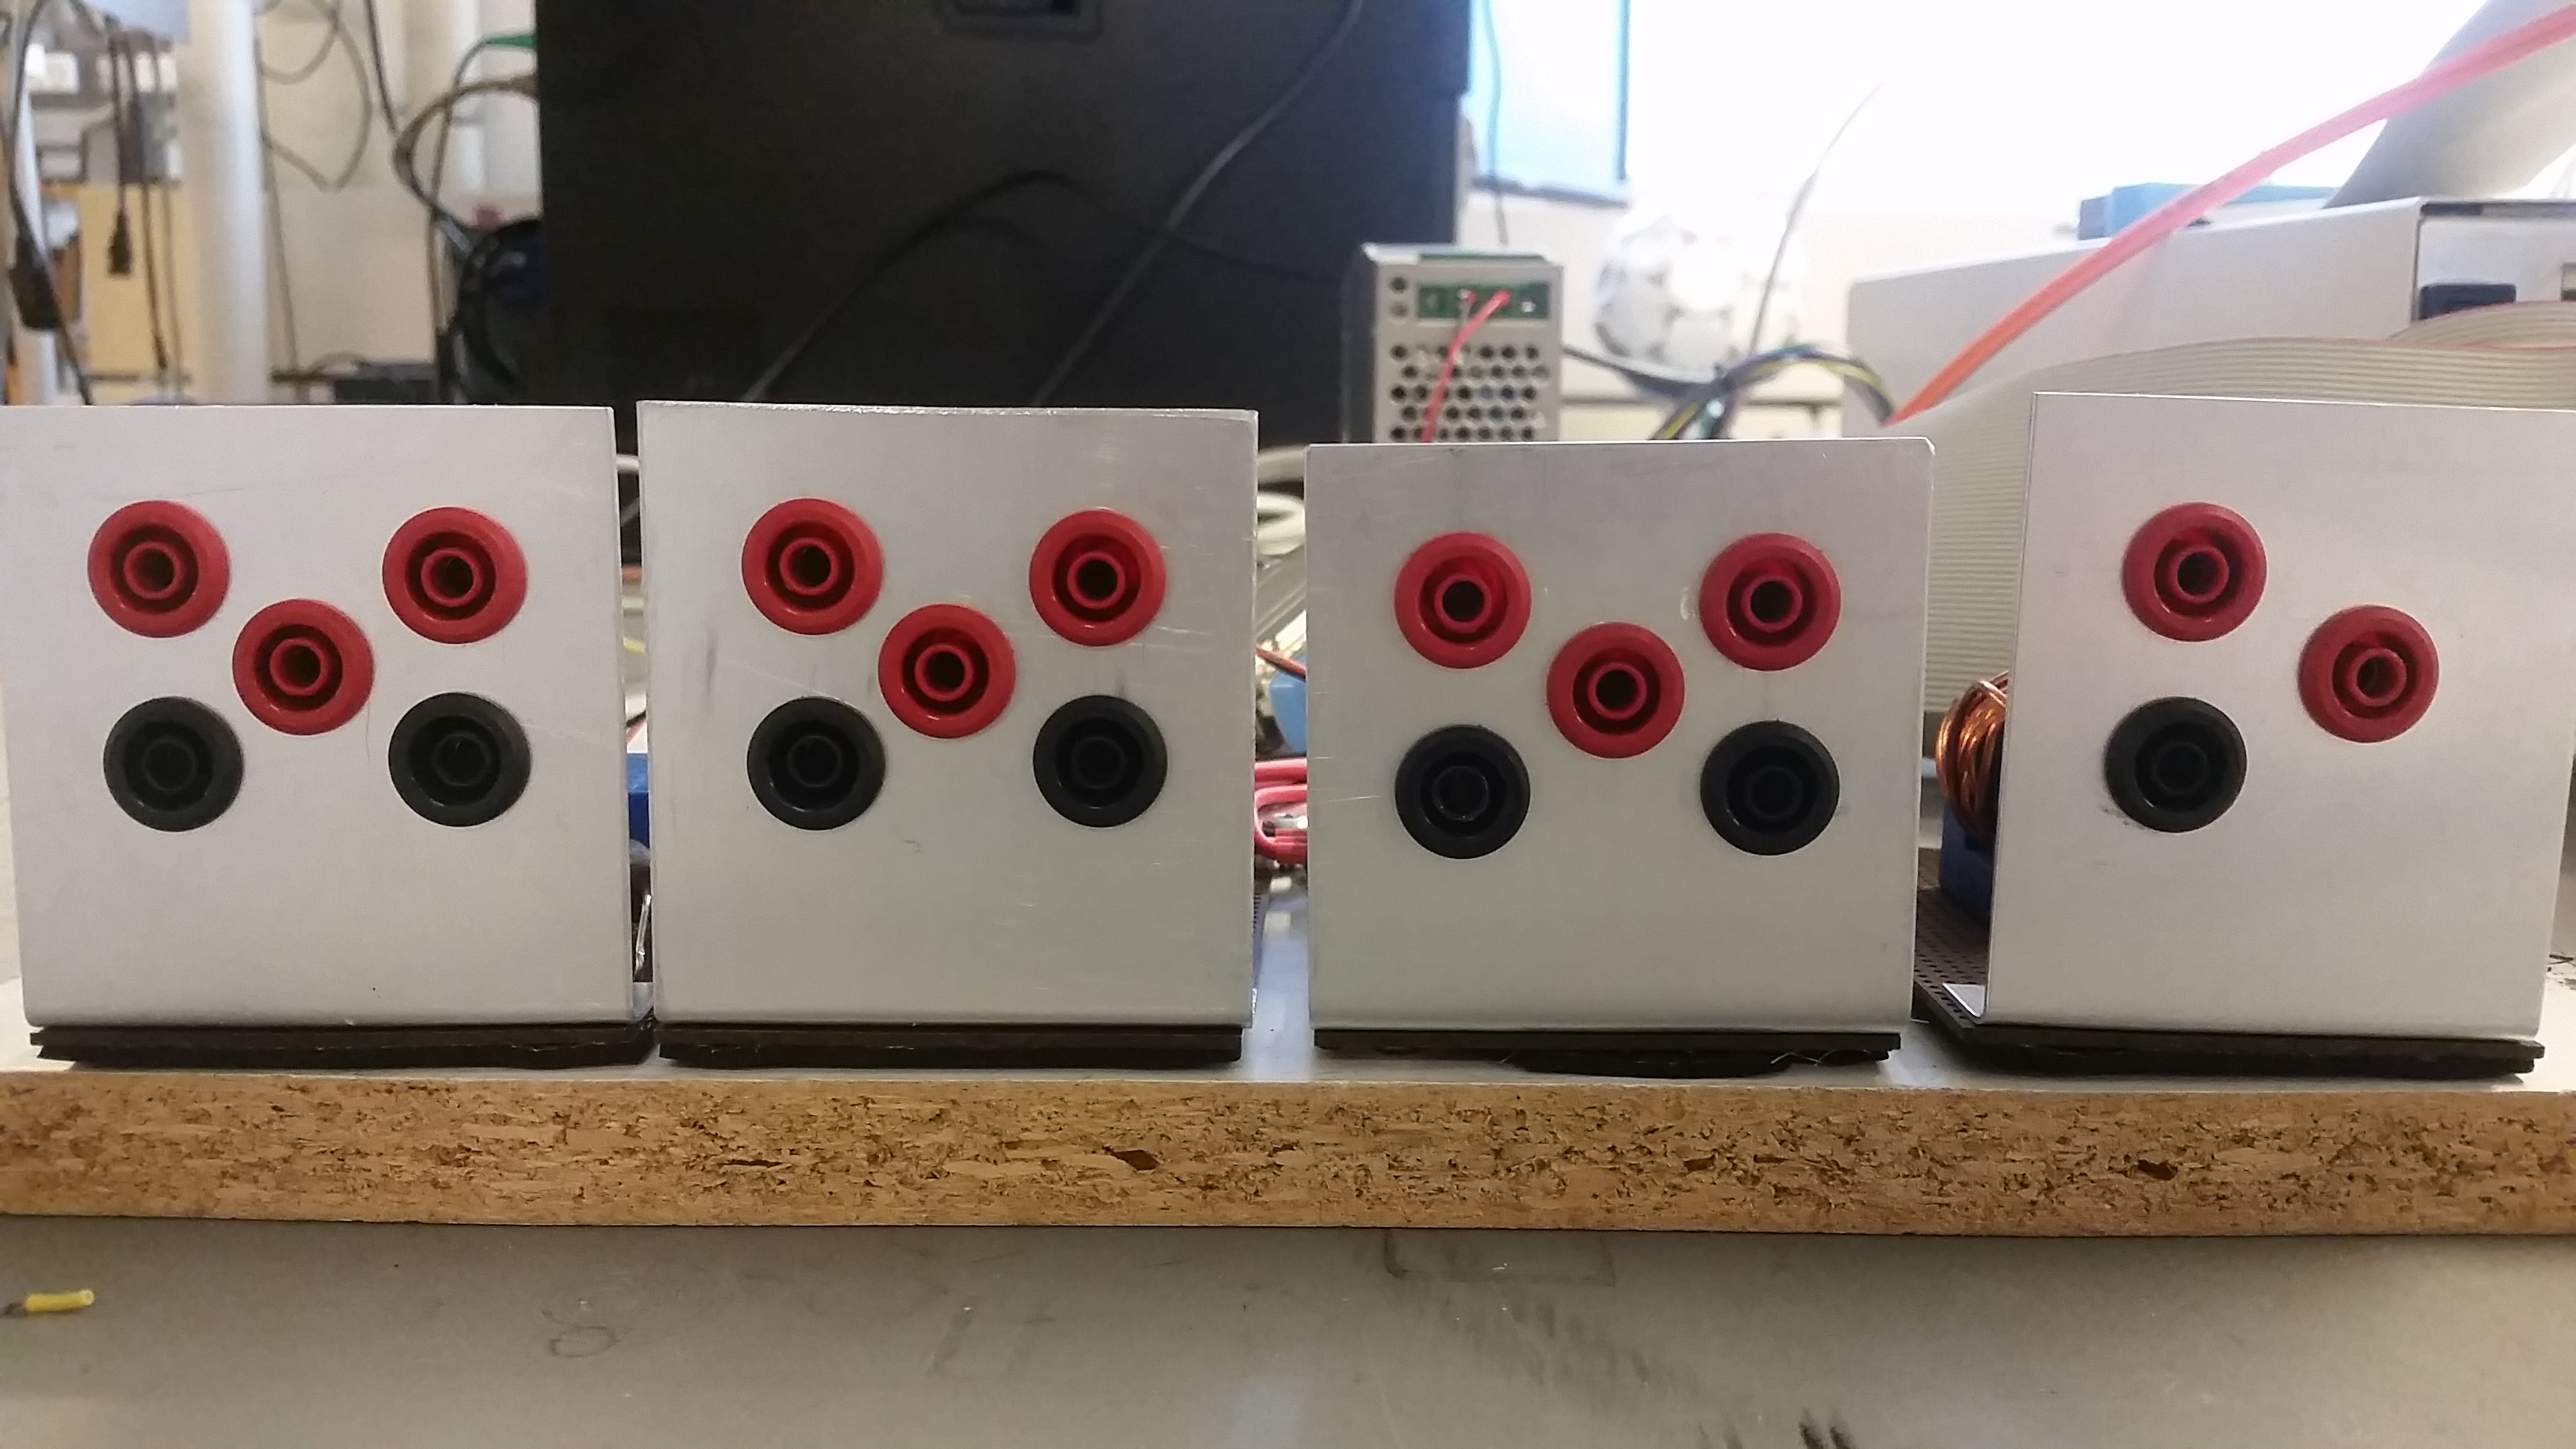
\includegraphics[width=1.5\textwidth]{rapport/billeder/Voltage_Current}
%   \caption{}
% \end{subfigure}
% \caption{(a) The dSPACE unit. (b) Voltage and current measurement inputs.   }
% \label{fig:dspace_voltage_current}
% \end{figure}

% On the backside of the dSPACE unit, there is placed the connections for communication with PC and the connection to all the boards that are placed on the wooden plate. In \figref{fig:dspace_voltage_current} b the voltage and current measurements inputs are shown. There are placed four current measurements which is able to measure current from ?? to ?? and from ?? to ?? \fxnote{Hear Jesper what the size of the current measurement}. It is also able to measure three different voltage signals. 

% \begin{figure}[H]
% \centering
% 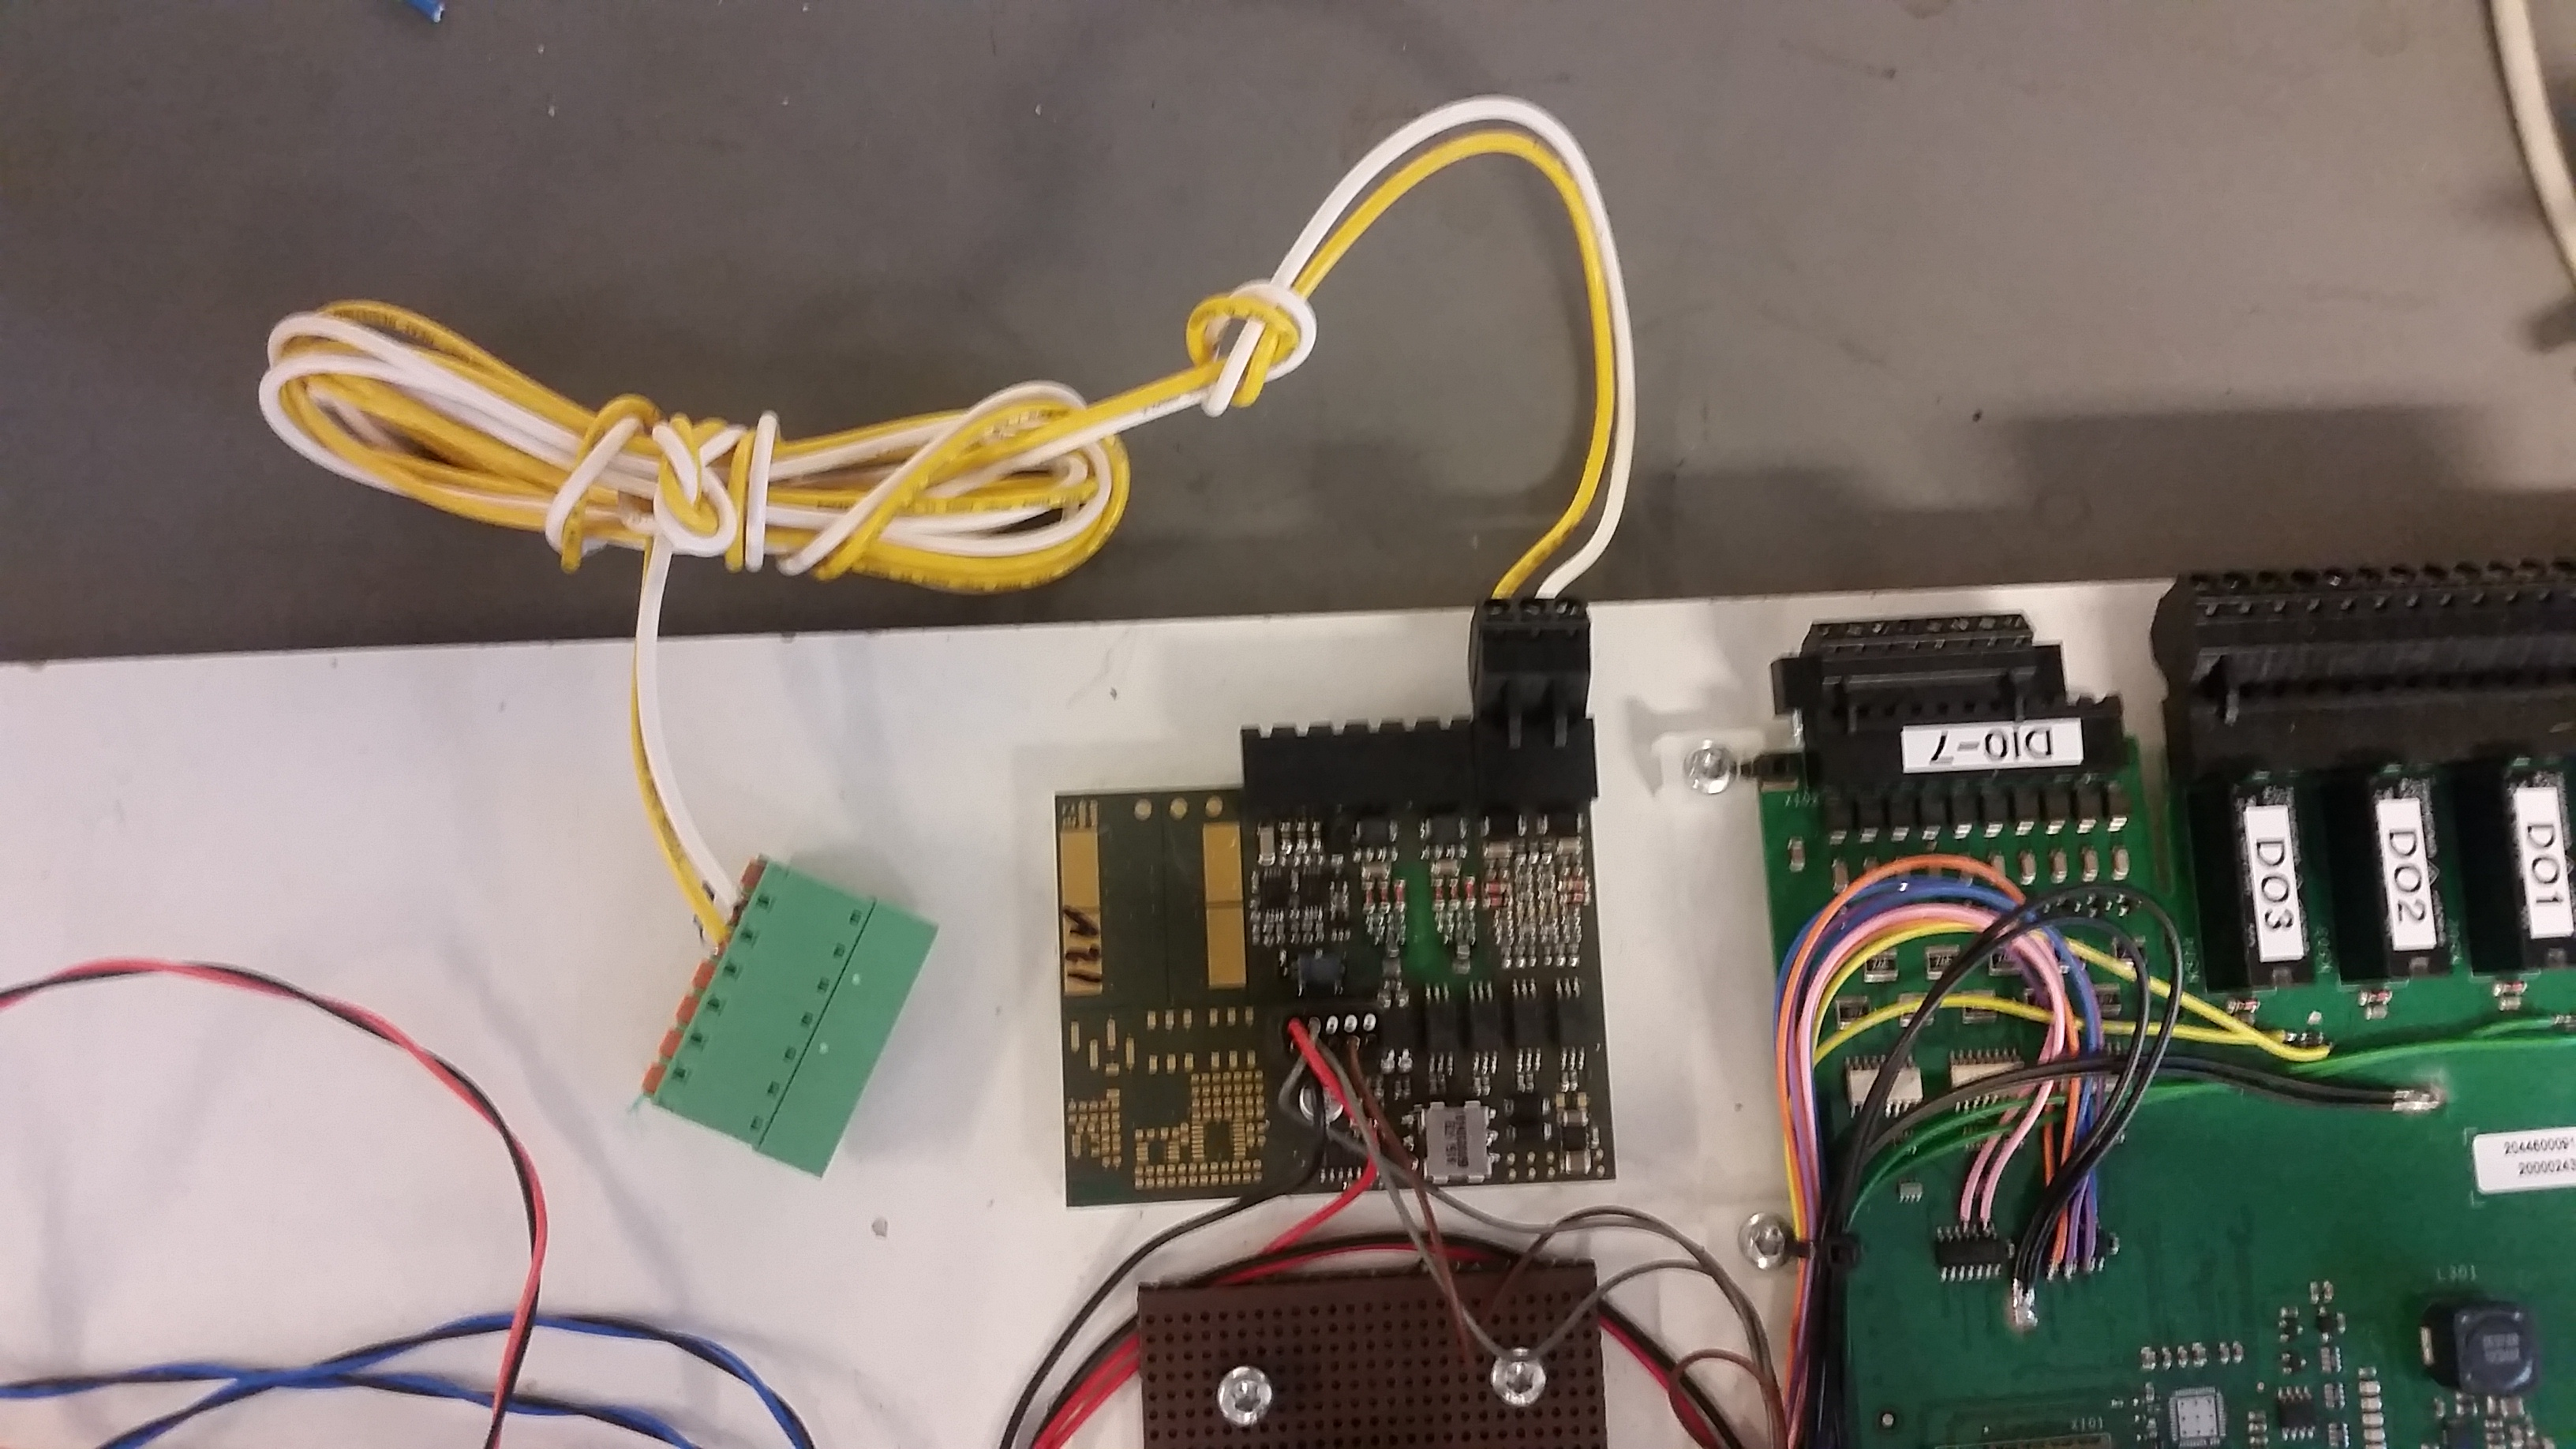
\includegraphics[width=0.50\textwidth]{rapport/billeder/frequence_interrupt}
% \caption{For measuring frequency.}
% \label{fig:CAN_arbitration}
% \end{figure}    

% \fxnote{Need something to call this board} This board is able to receive interrupts from the the genset, which can be used to calculated the electric frequency. I need to elaborate this. (Jacob)

% To implement the controller, simulink is used with a dSPACE toolbox.  

% Something on the overall system like the compelete setup with computer and wooden board

% Break down in smaller piceses(stykker) start with the board 

% Go into the simulink files

% End with the matlab file

% Maybe our controller implemented in simulink. 

% \begin{figure}[H]
% \centering
% 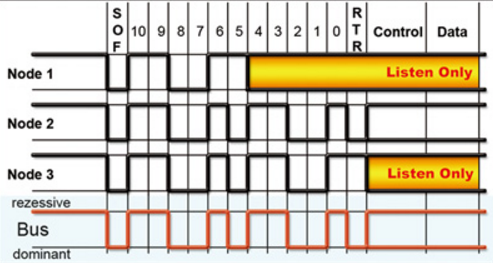
\includegraphics[width=0.75\textwidth]{rapport/billeder/CAN_arbitration}
% \caption{Showing arbitration behavior on a CAN bus \cite{fig_CAN_arbitation}.}
% \label{fig:CAN_arbitration}
% \end{figure}